% Created by tikzDevice version 0.12 on 2019-06-14 18:13:08
% !TEX encoding = UTF-8 Unicode
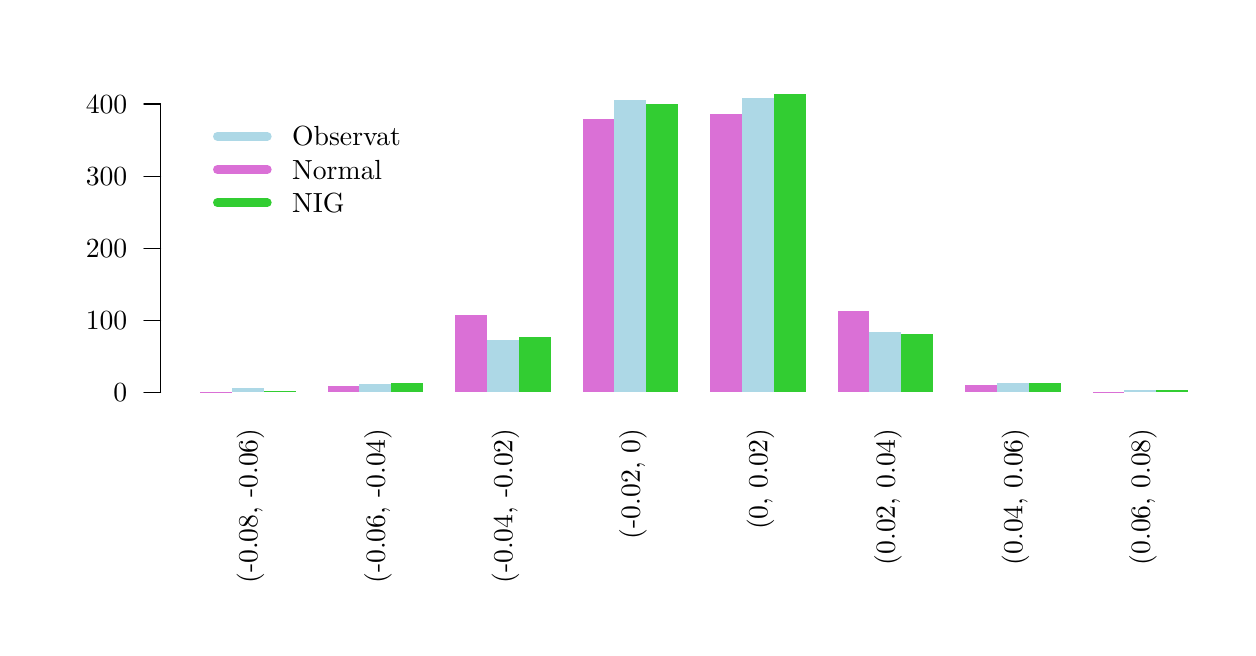
\begin{tikzpicture}[x=1pt,y=1pt]
\definecolor{fillColor}{RGB}{255,255,255}
\path[use as bounding box,fill=fillColor,fill opacity=0.00] (0,0) rectangle (433.62,216.81);
\begin{scope}
\path[clip] (  0.00,  0.00) rectangle (433.62,216.81);
\definecolor{fillColor}{RGB}{218,112,214}

\path[fill=fillColor] ( 62.28, 85.08) rectangle ( 73.80, 85.12);
\definecolor{fillColor}{RGB}{173,216,230}

\path[fill=fillColor] ( 73.80, 85.08) rectangle ( 85.32, 86.64);
\definecolor{fillColor}{RGB}{50,205,50}

\path[fill=fillColor] ( 85.32, 85.08) rectangle ( 96.84, 85.69);
\definecolor{fillColor}{RGB}{218,112,214}

\path[fill=fillColor] (108.35, 85.08) rectangle (119.87, 87.28);
\definecolor{fillColor}{RGB}{173,216,230}

\path[fill=fillColor] (119.87, 85.08) rectangle (131.39, 87.94);
\definecolor{fillColor}{RGB}{50,205,50}

\path[fill=fillColor] (131.39, 85.08) rectangle (142.91, 88.35);
\definecolor{fillColor}{RGB}{218,112,214}

\path[fill=fillColor] (154.43, 85.08) rectangle (165.94,112.90);
\definecolor{fillColor}{RGB}{173,216,230}

\path[fill=fillColor] (165.94, 85.08) rectangle (177.46,103.82);
\definecolor{fillColor}{RGB}{50,205,50}

\path[fill=fillColor] (177.46, 85.08) rectangle (188.98,105.05);
\definecolor{fillColor}{RGB}{218,112,214}

\path[fill=fillColor] (200.50, 85.08) rectangle (212.02,183.78);
\definecolor{fillColor}{RGB}{173,216,230}

\path[fill=fillColor] (212.02, 85.08) rectangle (223.53,190.78);
\definecolor{fillColor}{RGB}{50,205,50}

\path[fill=fillColor] (223.53, 85.08) rectangle (235.05,189.28);
\definecolor{fillColor}{RGB}{218,112,214}

\path[fill=fillColor] (246.57, 85.08) rectangle (258.09,185.71);
\definecolor{fillColor}{RGB}{173,216,230}

\path[fill=fillColor] (258.09, 85.08) rectangle (269.60,191.56);
\definecolor{fillColor}{RGB}{50,205,50}

\path[fill=fillColor] (269.60, 85.08) rectangle (281.12,192.81);
\definecolor{fillColor}{RGB}{218,112,214}

\path[fill=fillColor] (292.64, 85.08) rectangle (304.16,114.57);
\definecolor{fillColor}{RGB}{173,216,230}

\path[fill=fillColor] (304.16, 85.08) rectangle (315.68,106.95);
\definecolor{fillColor}{RGB}{50,205,50}

\path[fill=fillColor] (315.68, 85.08) rectangle (327.19,106.24);
\definecolor{fillColor}{RGB}{218,112,214}

\path[fill=fillColor] (338.71, 85.08) rectangle (350.23, 87.51);
\definecolor{fillColor}{RGB}{173,216,230}

\path[fill=fillColor] (350.23, 85.08) rectangle (361.75, 88.46);
\definecolor{fillColor}{RGB}{50,205,50}

\path[fill=fillColor] (361.75, 85.08) rectangle (373.27, 88.54);
\definecolor{fillColor}{RGB}{218,112,214}

\path[fill=fillColor] (384.78, 85.08) rectangle (396.30, 85.13);
\definecolor{fillColor}{RGB}{173,216,230}

\path[fill=fillColor] (396.30, 85.08) rectangle (407.82, 85.86);
\definecolor{fillColor}{RGB}{50,205,50}

\path[fill=fillColor] (407.82, 85.08) rectangle (419.34, 85.72);
\end{scope}
\begin{scope}
\path[clip] (  0.00,  0.00) rectangle (433.62,216.81);
\definecolor{drawColor}{RGB}{0,0,0}

\node[text=drawColor,rotate= 90.00,anchor=base east,inner sep=0pt, outer sep=0pt, scale=  1.00] at ( 83.00, 72.00) {(-0.08, -0.06)};

\node[text=drawColor,rotate= 90.00,anchor=base east,inner sep=0pt, outer sep=0pt, scale=  1.00] at (129.07, 72.00) {(-0.06, -0.04)};

\node[text=drawColor,rotate= 90.00,anchor=base east,inner sep=0pt, outer sep=0pt, scale=  1.00] at (175.15, 72.00) {(-0.04, -0.02)};

\node[text=drawColor,rotate= 90.00,anchor=base east,inner sep=0pt, outer sep=0pt, scale=  1.00] at (221.22, 72.00) {(-0.02, 0)};

\node[text=drawColor,rotate= 90.00,anchor=base east,inner sep=0pt, outer sep=0pt, scale=  1.00] at (267.29, 72.00) {(0, 0.02)};

\node[text=drawColor,rotate= 90.00,anchor=base east,inner sep=0pt, outer sep=0pt, scale=  1.00] at (313.36, 72.00) {(0.02, 0.04)};

\node[text=drawColor,rotate= 90.00,anchor=base east,inner sep=0pt, outer sep=0pt, scale=  1.00] at (359.43, 72.00) {(0.04, 0.06)};

\node[text=drawColor,rotate= 90.00,anchor=base east,inner sep=0pt, outer sep=0pt, scale=  1.00] at (405.50, 72.00) {(0.06, 0.08)};

\path[draw=drawColor,line width= 0.4pt,line join=round,line cap=round] ( 48.00, 85.08) -- ( 48.00,189.22);

\path[draw=drawColor,line width= 0.4pt,line join=round,line cap=round] ( 48.00, 85.08) -- ( 42.00, 85.08);

\path[draw=drawColor,line width= 0.4pt,line join=round,line cap=round] ( 48.00,111.11) -- ( 42.00,111.11);

\path[draw=drawColor,line width= 0.4pt,line join=round,line cap=round] ( 48.00,137.15) -- ( 42.00,137.15);

\path[draw=drawColor,line width= 0.4pt,line join=round,line cap=round] ( 48.00,163.19) -- ( 42.00,163.19);

\path[draw=drawColor,line width= 0.4pt,line join=round,line cap=round] ( 48.00,189.22) -- ( 42.00,189.22);

\node[text=drawColor,anchor=base east,inner sep=0pt, outer sep=0pt, scale=  1.00] at ( 36.00, 81.63) {0};

\node[text=drawColor,anchor=base east,inner sep=0pt, outer sep=0pt, scale=  1.00] at ( 36.00,107.67) {100};

\node[text=drawColor,anchor=base east,inner sep=0pt, outer sep=0pt, scale=  1.00] at ( 36.00,133.71) {200};

\node[text=drawColor,anchor=base east,inner sep=0pt, outer sep=0pt, scale=  1.00] at ( 36.00,159.74) {300};

\node[text=drawColor,anchor=base east,inner sep=0pt, outer sep=0pt, scale=  1.00] at ( 36.00,185.78) {400};
\end{scope}
\begin{scope}
\path[clip] ( 48.00, 84.00) rectangle (433.62,192.81);

\path[] ( 59.57,189.55) rectangle (139.31,141.55);
\definecolor{drawColor}{RGB}{173,216,230}

\path[draw=drawColor,line width= 3.2pt,line join=round,line cap=round] ( 68.57,177.55) -- ( 86.57,177.55);
\definecolor{drawColor}{RGB}{218,112,214}

\path[draw=drawColor,line width= 3.2pt,line join=round,line cap=round] ( 68.57,165.55) -- ( 86.57,165.55);
\definecolor{drawColor}{RGB}{50,205,50}

\path[draw=drawColor,line width= 3.2pt,line join=round,line cap=round] ( 68.57,153.55) -- ( 86.57,153.55);
\definecolor{drawColor}{RGB}{0,0,0}

\node[text=drawColor,anchor=base west,inner sep=0pt, outer sep=0pt, scale=  1.00] at ( 95.57,174.10) {Observat};

\node[text=drawColor,anchor=base west,inner sep=0pt, outer sep=0pt, scale=  1.00] at ( 95.57,162.10) {Normal};

\node[text=drawColor,anchor=base west,inner sep=0pt, outer sep=0pt, scale=  1.00] at ( 95.57,150.10) {NIG};
\end{scope}
\end{tikzpicture}
